\usetikzlibrary{arrows.meta, positioning}


\chapter{Process Mining}

With the increasing complexity of modern day \ac{erp} systems, it has become a challenge to document all the business logic and processes that take place in such a system \cite{dumas_laRosa_mendling_reijers_2018}. Process Mining with its self-generating charts and documentations from existing datasets of such systems is a potential solution to this problem. Initial Research on Process Mining was performed by Jonathan E. Cook with his paper ``Automated Process Discovery through Event-Data Analysis'' in the year of 1996. Another important researcher on Process Mining is \textbf{\citeauthor{AalstSpaghetti}}, who worked with many other researchers on the ``Process Mining Manifesto'' in 2012. In this work, Process Mining is positioned as being closely related to Data Mining, which focuses on extracting insights from large datasets \cite{processminingmanifesto}.

To understand the relationship between information systems and Process Mining, three fundamental concepts are introduced: \textit{play-in}, \textit{play-out}, and \textit{replay} \cite{vanDerAalst2012ProcessMiningOverview}. \textit{Play-out} refers to the classical use of process models. After a process is executed, the execution log contains all traces from the prior execution. When a software system manages and executes processes involving people, applications, or information sources, it is called a  \ac{pais}. \ac{pais} therefore can be seen as \textit{play-out} engines, which create traces according to the model \cite{AalstSpaghetti, ReichertWeber2012}. \textit{Play-in} marks the  opposite, as it uses an event log to create a process model \cite{vanderAalst2016_processmining_in_action}.
\textit{Replay} on the other side uses both an event log and a process model. The event log is played ``on top'' in comparison to the process model to find deviations and mismatches. Use Cases of replaying the model might be conformance checking, building predictive models and operational support (e.g. alerting) \cite{ReichertWeber2012}. 

Process Mining is based on on the general idea of Petri Nets \cite{Weske2024}. They are an important basis for process languages. They consist of places (can be seen as preconditions or states), transitions (actions or activities), and directed edges connecting places and transitions. An example can be seen in figure \ref{fig:petrinet}. 

The dynamic behavior of Petri Nets is represented by tokens and markings that run through the net while executing. Places can store one or multiple tokens, depending on the Petri Net type.  A transition fires if it is enabled \cite{ReichertWeber2012}. These Petri Nets now allow working with the execution log of e.g. a \ac{pais}. As Process Mining first started with Process Discovery, today it is combined with  Machine Learning to address inefficiencies and deviations \cite{reinkemeyer:2020}. 
In comparison to the \textit{data-centric} Data Mining, Process Mining  is \textit{process-centric} and focuses on \textit{fact-based} and \textit{truly-intelligence} analysis \cite{ReichertWeber2012}.


\begin{figure}%[h]
\centering
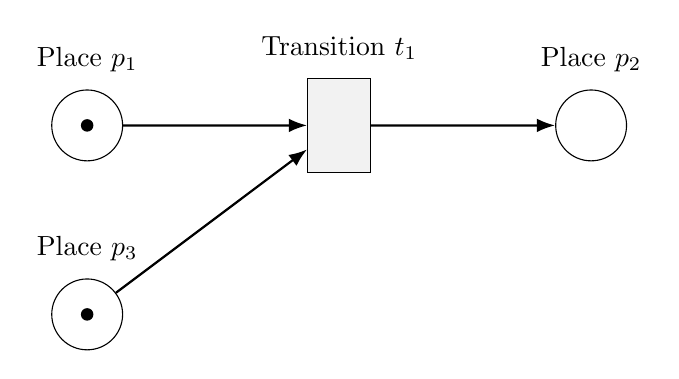
\begin{tikzpicture}[node distance=22mm, scale=0.8]

\tikzset{
  place/.style={circle, draw, minimum size=9mm, inner sep=0pt},
  transition/.style={rectangle, draw, minimum height=12mm, minimum width=8mm, fill=gray!10},
  token/.style={circle, fill=black, inner sep=1.6pt},
  >={Latex}
}

% Rest unverändert
% --- Titel / Kontext ---


% --- Netz-Knoten (mit absoluten Koordinaten) ---
\node[place] (p1) at (-8,1.5) {}; 
\node[transition] (t1) at (-4,1.5){}; 
\node[place] (p2) at (0,1.5) {}; 
\node[place] (p3) at (-8,-1.5) {}; 



%\node[place]      (p1) at (-10,-1.5)  {};   % erster Place links oben
%\node[transition] (t1) at (2.2,-1.5) {};  % erste Transition rechts davon
%\node[place]      (p2) at (4.4,-1.5) {};  % zweiter Place
%\node[transition] (t2) at (6.6,-1.5) {};  % zweite Transition
%\node[place]      (p3) at (8.8,-1.5) {};  % dritter Place



% --- Kanten ---
\draw[->, thick] (p1) -- (t1);
\draw[->, thick] (t1) -- (p2);
\draw[->, thick] (p3) -- (t1);


% --- Token als Markierung ---
\node[token] at (p1) {};
\node[token] at (p3) {};


% --- Beschriftungen ---
\node[above=1mm of p1] {Place $p_1$};
\node[above=1mm of t1] {Transition $t_1$};
\node[above=1mm of p2] {Place $p_2$};
\node[above=1mm of p3] {Place $p_3$};



\end{tikzpicture}

\caption{Petri Net Example with three Places and a Transition}
\label{fig:petrinet}
\end{figure}


%
%
\section{Event Log}

As already mentioned, the execution of one or several processes can be logged. This most essential part of process mining is the so-called \textbf{event log}. The execution log can be used for multiple purposes, such as monitoring, ensuring traceability, analysis as well as diagnosis \cite{ReichertWeber2012, Weske2024}. 
A minimum event log typically exists of three different columns, namely \textit{Case ID}, \textit{Activity} and \textit{Timestamp}. \textit{A User ID} is also beneficial and often mentioned, an example can be seen in table \ref{tab:minimal_event_log} \cite{ReichertWeber2012, reinkemeyer:2020}.   \\

\begin{table}[h]
\centering
\begin{tabular}{l | l | l| l}
\textbf{Case ID} & \textbf{Activity} & \textbf{Timestamp} & \textbf{User ID} \\
\hline
C01 & Approve Request & 2024-05-03 09:15 & U123 \\
\hline
C01 & Send Notification & 2024-05-03 09:18 & U088 \\
\hline
C02 & Validate Data & 2024-05-04 14:02 & U123 \\
\end{tabular}
\caption{Example of a minimal event log \cite{ReichertWeber2012}}
\label{tab:minimal_event_log}
\end{table}
\label{sec:lasagneshaphetti}

\newpage

Multiple instances of a Case ID are called a \textit{trace}, meaning a sequential flow of activities ordered by timestamp. 
In general, processes can be distinguished into two separated groups based on their complexity \cite{vanDerAalst2012ProcessMiningOverview}. One group, containing very complex and hard to follow process charts, is called \textit{spaghetti process}. The complexity reflexes the reality shown in the log files, hence it is not caused by the discovery algorithm, and the model is too complex to understand \cite{AalstSpaghetti}. The second category is called \textit{lasagna process} and describes the very opposite: highly structured, easy to understand, and displayable processes \cite{vanDerAalst2012ProcessMiningOverview}. 


\begin{figure}%[h]
\centering
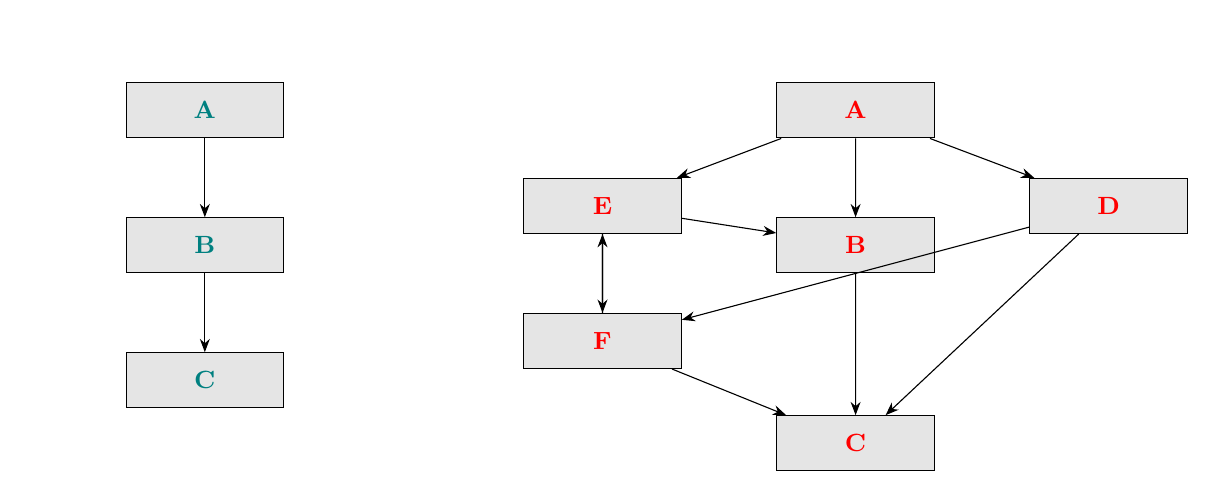
\begin{tikzpicture}[scale=0.7,
    every node/.style={draw, fill=gray!20, minimum width=2cm, minimum height=0.7cm, font=\small},
    >=Stealth]

% Linkes Diagramm
\node[draw=none, fill=none, minimum size=4.5cm, thick, teal, circle] (C1) {};
\node (A1) at (C1.center) [yshift=1.2cm] {\textcolor{teal}{\textbf{A}}};
\node (M1) [below=of A1] {\textcolor{teal}{\textbf{B}}};
\node (B1) [below=of M1] {\textcolor{teal}{\textbf{C}}};

\draw[->] (A1) -- (M1);
\draw[->] (M1) -- (B1);

% Untertitel (a)
%\node[draw=none, fill=none, below=0.4cm of B1, font=\small] {(a) Linear};

% Rechtes Diagramm
\node[draw=none, fill=none, minimum size=4.5cm, thick, red, circle, right=6cm of C1.center] (C2) {};
\node (A2) at (C2.center) [yshift=1.2cm] {\textcolor{red}{\textbf{A}}};
\node (N1) [below=of A2] {\textcolor{red}{\textbf{B}}};
\node (N2) [below right=0.5cm and 1.2cm of A2] {\textcolor{red}{\textbf{D}}};
\node (N3) [below left=0.5cm and 1.2cm of A2] {\textcolor{red}{\textbf{E}}};
\node (N4) [below=of N3] {\textcolor{red}{\textbf{F}}};
\node (B2) [below=of N1, yshift=-0.8cm] {\textcolor{red}{\textbf{C}}};

% Pfeile
\draw[->] (A2) -- (N1);
\draw[->] (A2) -- (N2);
\draw[->] (A2) -- (N3);
\draw[->] (N1) -- (B2);
\draw[->] (N3) -- (N4);
\draw[->] (N4) -- (B2);
\draw[->] (N2) -- (B2);
\draw[->] (N2) -- (N4);
\draw[->] (N3) -- (N1);
\draw[->] (N4) -- (N3);

% Untertitel (b)
%\node[draw=none, fill=none, below=0.4cm of B2, font=\small] {(b) Vernetzt};

\end{tikzpicture}
\caption{Expected Process vs. Process in Reality \cite{vanDerAalst2012ProcessMiningOverview}}
\label{fig_expectedprocess_vs_reality}
\end{figure}

By design, processes are supposed to follow a strict set of events (see process on the left in figure \ref{fig_expectedprocess_vs_reality}), however they often turn out to be more complex (see figure \ref{fig_expectedprocess_vs_reality} on the right) \cite{reinkemeyer:2020}. Reasons to this can be diverse, e.g. manual input, exception handling or errors inside the workflow engine \cite{vanDerAalst2012ProcessMiningOverview}. 

\newpage

\section{Quality Criteria}
There are in total six different quality criteria that can be assigned to process models to rate either the \textbf{quality of the event log} or the \textbf{quality of the process model} \cite{ReichertWeber2012}.

\subsection{Event Log}
Regarding quality of the event log, to \citeauthor{AalstSpaghetti} the selected log must contain a 
\begin{quote}
\textit{``representative sample of the model behavior.''} \cite{vanderAalst2016_processmining_in_action}
\end{quote}
Otherwise, conclusions of the process model cannot be made based on the event log since it is lacking information. \citeauthor{vanderAalst2016_processmining_in_action} mentions two different quality criteria for event logs: 

\textbf{Noise} describes a phenomenon where the event log contains traces that never or only very rarely happen in the real world. This does not refer to incorrect logging, more so there might be human input, interruption, or error handling. The evolving term of the $80/20$ model describes an ideal situation where $80\%$ of the behavior of the process model can be described by only $20\%$ of the variability of the event log. The remaining $80\%$    of the variability only makes up $20\%$ of the behavior and therefore can be seen as negligible \cite{vanderAalst2016_processmining_in_action}.

\textbf{Incompleteness} describes a phenomenon where the event log contains too few traces to create a process model that reflects reality. As real-world process models typically allow for thousands 
of different traces, it is unrealistic to assume that every possible trace is part of the event log \cite{vanderAalst2016_processmining_in_action, ReichertWeber2012}.

\newpage
\label{sec:quality_criteria}
\subsection{Process Modeling}
In process modeling, four fundamental and mutually competing quality criteria are typically considered: \textit{fitness}, \textit{simplicity}, \textit{precision}, and \textit{generalization} \cite{vanderAalst2011ProcessMining}. These criteria capture different aspects of model quality and are often in tension with one another, such that improvements in one dimension may lead to trade-offs in others. The construction of high-quality process models therefore requires a balanced consideration of all four criteria \cite{reinkemeyer:2020}. As shown in Figure \ref{fig:four_quality_dimensions}, \textit{fitness} measures how well a model can replay the observed event log, while \textit{precision} indicates how strictly the model restricts behavior to what is actually observed. In contrast, \textit{generalization} reflects the ability to allow plausible but unseen behavior, and \textit{simplicity} follows the principle of Occam’s razor by favoring models that are easy to understand. High-quality process models aim to balance these four criteria rather than optimizing any single one in isolation \cite{vanderAalst2011ProcessMining, Buijs2014DiscoveringNavigating}. 

\begin{figure}
    \centering
 
\begin{tikzpicture}[
    >=Stealth,
    every node/.style={align=center},
    arrow/.style={->, thick, gray}
]

% Zentrales Oval
\node[draw, ellipse, thick, minimum width=4cm, minimum height=2cm] (pd) {
    \textbf{process}\\
    \textbf{discovery}
};

% Oben links: replay fitness
\node[above left=0.5cm and 1cm of pd] (fitness) {
    ``able to replay event log''\\
    \textbf{replay fitness}
};
\draw[arrow] (pd) -- (fitness);

% Oben rechts: simplicity
\node[above right=0.5cm and 1.5cm of pd] (simplicity) {
    ``Occam's razor''\\
    \textbf{simplicity}
};
\draw[arrow] (pd) -- (simplicity);

% Unten links: generalization
\node[below left=0.5cm and 1cm of pd] (generalization) {
    \textbf{generalization}\\
    ``not overfitting the log''
};
\draw[arrow] (pd) -- (generalization);

% Unten rechts: precision
\node[below right=0.5cm and 1cm of pd] (precision) {
    \textbf{precision}\\
    ``not underfitting the log''
};
\draw[arrow] (pd) -- (precision);

\end{tikzpicture}
    \caption{Four Quality Dimensions of Process Discovery \cite{vanderAalst2011ProcessMining}}
    \label{fig:four_quality_dimensions}
\end{figure}


\section{Kinds of Process Ming}

In general, process mining is commonly divided into \textbf{process discovery}, \textbf{conformance checking}, and \textbf{process enhancement} \cite{vanderAalst2011ProcessMining, ReichertWeber2012, reinkemeyer:2020}. These three categories address different stages of the process lifecycle, ranging from the automated construction of process models from event data to the analysis and improvement of existing processes.


\subsection{Discovery}

Marking the original cause of Process Mining, Process Discovery  aims to automatically construct process models from event data without any prior knowledge of the underlying process structure. The goal is to derive a formal representation, such as a Petri net or \ac{bpmn} diagram, that captures the behavior recorded in the event log as accurately as possible \cite{dumas_laRosa_mendling_reijers_2018}.
Unlike traditional process modeling, which depends on interviews, documentation, and manual analysis, Process Discovery relies on empirical event data that reflect how processes are executed in reality \cite{vanderAalst2011ProcessMining}.

For example, \citeauthor{dumas_laRosa_mendling_reijers_2018} define general process discovery as 
\begin{quote}
    

\textit{``the act of gathering information about an existing process and organizing it.''} \cite{dumas_laRosa_mendling_reijers_2018} 

\end{quote}
and mention evidence-, interview- and workshop-based discovery. All three presume that involved people are familiar with the process. To overcome this dependency on subjective human input, Process Mining enables an automated form of process discovery based on execution logs. It can be used if the execution log is already present which is mined afterwards, no matter by hand or by an algorithm \cite{dumas_laRosa_mendling_reijers_2018, ReichertWeber2012}. This makes it a data-driven approach capable of uncovering deviations, hidden workflows, or bottlenecks that may not be apparent in the designed process models \cite{Bernard2016SalesProcessMining}. Problems come along when the process changes over time which may result in incorrect process models build by the discovery algorithm. To address this issue, there are techniques that try to identify different versions of the process \cite{ReichertWeber2012}.

\newpage 
Process Discovery techniques can be broadly divided into bottom-up and top-down approaches \cite{vanderAalst2022ProcessMiningHandbook}:
\begin{enumerate}
    \item \textbf{Bottom-up discovery} approaches start from the local relations between activities in the event log and build up the model incrementally. One of the most influential methods in this category is the $\alpha$-algorithm, introduced by van der Aalst and Weijters, which identifies relationships between activities based on their ordering in traces \cite{vanderAalst2011ProcessMining, vanderAalst2016_processmining_in_action}. However, it is vulnerable to noise \cite{OrtmeierFrameworkIntoLifeCycleAssessment}. 
    \item \textbf{Top-down discovery} approaches construct process models from a global perspective by continuously breaking down the event log into smaller versions. Inductive mining algorithms are a prominent example of this category \cite{OrtmeierFrameworkIntoLifeCycleAssessment}. Because they are more resilient to noise, they ensure the discovery of sound, block-structured models, which makes them suitable for more complex real-world applications \cite{vanderAalst2022ProcessMiningHandbook}.
\end{enumerate}

In business context, Process Discovery can be used on processes itself, on organizations perspectives, on social networks or staff aissignment rules \cite{ReichertWeber2012}.
A key aspect of modern Process Discovery is the trade-off between the already mentioned quality criteria in chapter \ref{sec:quality_criteria} \cite{AalstSpaghetti}. 

\subsection{Conformance}
Conformance checking deals with the analysis how far an execution log matches a given process model. Specifically, it can highlight discrepancies and therefore show problems that come along after real executions \cite{vanderAalst2022ProcessMiningHandbook, ReichertWeber2012}. It is relevant for business alignment and auditing. Conformance checking allows to create \ac{kpi}s such as \textit{"$85\%$ of the cases in this event log can be replayed by the model"} (compare \cite{ReichertWeber2012}). How the missing $15\%$ can be interpreted, depends on the use case. 

\citeauthor{AalstSpaghetti} introduces the two terms \textit{descriptive} and \textit{normative}. If the model can be seen descriptive, it needs to be changed to reach the maximum, e.g. $100\%$ re-playability. If the model can be seen normative, one has to distinguish between \textit{undesirable deviations} and \textit{desirable deviations}. These two angles always need to be considered before taking actions to change the process model \cite{ReichertWeber2012}.



\subsection{Enhancement}
Enhancement uses extension algorithms to improve an existing process model based on information from the execution log. Enhancements can be, for example, better decisions based on past execution inside \ac{pais} such as removal of bottlenecks or unplanned behavior \cite{vanderAalst2022ProcessMiningHandbook, ReichertWeber2012}. \citeauthor{vanDerAalst2012ProcessMiningOverview} mentions that information from the event log can be extracted to identify roles of people, e.g. those who frequently perform tasks. Enhancement also allows to add data mining technics, such as decision trees to explain behavior or build social networks from work flows \cite{vanDerAalst2012ProcessMiningOverview, ReichertWeber2012}.

\clearpage
\section{L$^{\ast}$ Life-Cycle Model}

\begin{figure}
    \centering
    \includegraphics[width=1.09\linewidth]{images/L_lifecycle.png}
    \caption{The L$^{\ast}$ Life-Cycle Model \cite{AalstSpaghetti, Esiefarienrhe2021}}
    \label{fig:placeholder}
\end{figure}


The L$^{\ast}$ Life-Cycle Model is a framework designed to streamline process mining application on both spaghetti as well as lasagne processes which have already been introduced in section \ref{sec:lasagneshaphetti}\cite{Esiefarienrhe2021}. It was initially created by \citeauthor{AalstSpaghetti} in 2012. As spaghetti processes require a lot of manual work to structure and extract valuable information, a framework was needed to structure the optimal process mining project management \cite{AalstSpaghetti}. As multiple frameworks exist for the adoption of process mining into various fields such as lifecycle assessment (cf. \cite{OrtmeierFrameworkIntoLifeCycleAssessment}), a dedicated framework for lead management is yet to be introduced. 

The L$^{\ast}$ Life-Cycle Model is already adopted to business fields of flexible processes (e.g. the healthcare sector in \cite{Esiefarienrhe2021}) and therefore suitable for less structured processes \cite{OrtmeierFrameworkIntoLifeCycleAssessment}.

The framework is divided into five different stages, where most of them run sequentially. Nevertheless, the interpretation of results after the creation of control-flow and process models allows returning to earlier stages, thereby supporting an iterative approach.

Stage 0, called \textbf{plan and justify}, is supposed to build the foundation and motivation for the process mining project. Resources need to be allocated, project milestones defined and a team needs to be built up. Projects can be distinguished between three different types:

\begin{enumerate}
    \item The \textit{data-driven project} start without a concrete question in mind. Managers, stakeholders, and business analysts hope to find meaningful insights after analyzing the event log of the process. The project therefore has an explorative character \cite{Esiefarienrhe2021}. 
    \item A \textit{question-driven project} starts with initial questions and aims to answer these questions during analyzing the data. Beneficial is the fact that the analyst always has a goal in mind and is not distracted by the sheer amount of capabilities by modern-day process mining software \cite{AalstSpaghetti, Esiefarienrhe2021}. 
    \item A \textit{goal-driven project} sets \ac{kpi} and aims to improve these e.g. via cost reduction or improved throughput times \cite{Esiefarienrhe2021}. 
\end{enumerate}

\citeauthor{AalstSpaghetti} recommends companies without much process mining experience to start with \textit{question-driven} since it helps to streamline resources \cite{AalstSpaghetti}.

Stage 1, called \textbf{Extract}, deals with extracting event logs, objectives and questions from affected systems. This step may the be most time-consuming task. Van der Aalst names the example of SAP Systems, where relevant data is stored in thousands of tables and finding the correct data can be very challenging. If the company has some existing process models, they can be used to exploit existing knowledge. Inside stage 1, the objectives of a goal-driven process mining projects have to be defined, as well as the questions of a question-driven project.

Stage 2, called \textbf{Create Control-Flow Model and Connect Event Log} deals with creating the real-world control-flow via discovery algorithms such as $\alpha$ -algorithm, heurisitic miner or fuzzy miner. This discovered model can be evaluated by conformance checking against traces. Challenges during discovery can be overfitting, underfitting and representational bias of the selected algorithm. However more complex algorithms such as the heuristic miner can deal with these problems quite well \cite{Bernard2016SalesProcessMining}. Subsequent analysis should only be done if the model reaches a good fitness, meaning the discovered model can replay most of the traces. Van der Aalst recommends a fitness above 0.8, anything below is considered low \cite{AalstSpaghetti}. However this only applies to spaghetti processes, since lasagna processes can be fully modeled anyways. The results of stage 2 can be used to answer first questions of a question-driven project \cite{Esiefarienrhe2021}.

Stage 3, called \textbf{Create Integrated Process Model}, aims to add additional perspectives to the control flow model. One perspective can be organizational, meaning department and user-specific data. This organizational data can be used to e.g. identify bottlenecks via long throughput times. These insights can be used to make adjustments within the organization to address the bottleneck \cite{Esiefarienrhe2021}.

Stage 4, \textbf{Operational Support}, deals with detection, prediction and recommendation of the process. Running data is required to make predictions and recommend actions. One action can be automated alerting based on specific paths that were followed by that process. Predictions can be sent to the persons working on the case to boost handling time. Stage 4 of the L* Life-Cycle model is the most ambitious stage and requires advanced IT infrastructure and live data connection to the source system. It is also only possible for lasagna processes, since spaghetti processes cannot be designed to follow predictable paths \cite{AalstSpaghetti, Esiefarienrhe2021}.

